\documentclass{article}
\usepackage{graphicx}
\usepackage{float}
\usepackage{mathtools}

\author{}
\title{ELEC 302-81\\ Lab 5\\ Motor Torque, Speed, Losses, and Efficiency}
\date{\today}

\begin{document}

\maketitle

\begin{center}
  \begin{tabular}{lr}
    Date Performed: & February 25, 2013 \\
    Partners: & Rawley Dent \\
              & Charles Pittman \\
    Instructor: & Dr. Weatherford
  \end{tabular}
\end{center}

\pagebreak

\setlength\parindent{0pt}

\section{Purpose of Experiment}

In this experiment, the Prime Mover and Dynamometer modules were used to
measure torque, speed, power, and efficiency of a DC motor. This experiment
consisted of three parts. Part 1 involved only the Prime Mover module, and the
basic operation of the Prime Mover was studied and the friction torque
generated without a load was measured. Part 2 involved the Dynamometer acting
as a load to the Prime Mover, and the changes in torque due to the additon of
the Dynamometer were studied. Part 3 involved an experimental study of the
Prime Mover power losses and efficiency.

\section{Procedure}

\subsection{EMS Workstation Set-up}

The main power switch and voltage control knob were verified to be OFF and
fully counterclockwise, respectively. The voltmeter selector switch was set to
position 7--N. The Low Power Inputs for the Prime Mover/Dynamometer (PM/Dyno)
module and the Data Acquisition Interface (DAI) were connected to the 24-V
supply. The 24-V supply was turned on. The DAI USB was connected to the
computer. On the computer, the file for Lab 05 was opened in the EMS
application, and the metering window was set to continuous refresh.

\subsection{Prime Mover Operation}

\label{part1} The cicuit represented by Figure~\ref{fig:circuit_01} was
constructed. The Prime Mover module on the left side of the Prime
Mover/Dynamometer workstation was used in Part 1. Special, smaller sized
connection wires were used to connect the torque (T) and speed (N) terminals
from the PM/Dyno module to the DAI module. The white ground terminal was also
connected between the two modules. On the PM/Dyno control switches, the Mode
switch was set to Prime Mover (PM) and the Display switch was set to Speed (n).
The main voltage supply was turned ON and the DC supply voltage was adjuted to
30-V. Both the installed analog EMS voltmeter and the metering window were
monitored for proper indications. The DC voltage E1, the speed n indicated on
the Prime Mover digital display, and the speed N indicated on the computer
metering window were measured and recorded. The direction of rotation of the
prime mover was also recorded. These values are shown in
Table~\ref{tab:table_01}. On the PM/Dyno module, the Display switch was set to
the Torque position.  The friction torque, $T_f$, indicated on the Prime Mover
digital display and the Torque, $T$, indicated in the metering window were
measured and recorded. These values are also shown in Table~\ref{tab:table_01}.
On the PM/Dyno module, the Mode switch was set to the Dyn position. After a few
seconds, the Mode was set back to the PM position. The voltage control knob was
turned fully CCW and the main power switch was set to {OFF}.  The polarity of
the leads at the Prime Mover Input were then reversed. The main power switch
was turned ON and the voltage supply was adjusted to 30-V. The DC voltage E1,
the speed n indicated on the Prime Mover digital display, and the speed N
indicated on the computer metering window were measured and recorded. The
direction of rotation of the prime mover was also recorded. These values are
shown in Table~\ref{tab:table_01}. The voltage control knob was set fully CCW
and the main power switch to {OFF}. The leads were then connected to their
original polarity.

The power supply was set to {ON}. On the computer application, the Data Table
Applications window was opened. The Prime Mover Voltage, $E_1$, speed, $N$, and
torque, $T$, were checked as the values to be recorded in the table. Using the
voltage control knob, the Prime Mover speed was increased in approximately
300-rpm increments from 0--2100-rpm. At each 300- rpm increment, the values for
E1, N, and T were recorded into the Data Table. This data is shown in
Table~\ref{tab:table_02}. The voltage control knob was set fully CCW, and the
main power switch set to {OFF}. On the computer application, the Graph window
was opened. The Graph window was set to obtain a plot of Prime Mover Speed,
$N$, vs.  Prime Mover Voltage, $E_1$. The graph was created and then saved.
This graph is shown in Figure~\ref{fig:plot_01}. The graph window was then set
to obtain a plot of Prime Mover friction torque, $T$, vs. Prime Mover Speed
(rpm). The graph was created and then saved. This graph is shown in
Figure~\ref{fig:plot_02}.

\subsection{Dynamometer Operation}

\label{part2} A timing belt was used to couple the two modules of the PM/Dyno
together. The module on the left acted as the Prime Mover, and the module on
the right acted as the Dynamometer. The circuit represented by
Figure~\ref{fig:circuit_02} was constructed. The smaller sized leads were
connected to the T and N meters on the Dynamometer side. The 24-V supply was
connected to the PM/Dyno and the DAI modules. On the Prime Mover module, the
Mode switch was set to Prime Mover, and the Display switch was set to Speed. On
the Dynamometer module, the Mode switch was set to DYN, the Display switch was
set to Torque, the Load Control Mode switch was set to Man., and the Load
Control knob was set to Min. (fully CCW). The main power switch was set ON and
the voltage control knob was adjusted until to Prime Mover rotated at a speed
of 1500 rpm. On the Prime Mover module, the Display switch was set to Torque.
The opposition torque was then measured and recorded. This data is shown in
Table~\ref{tab:table_03}. The Display switch was returned to Speed. On the
Dynamometer module, the Load Control knob was slowly adjusted clockwise until
the torque on the digital dispay indicated 2.0 Nm. The voltage control knob was
then adjusted so that the Prime Mover rotated at 1500 rpm. The opposition
torque, $T_{PM}$, indicated by the Prime Mover digital display and the
non-corrected output torque, $T_{NC}$, in the metering window were measured and
recorded. These values are shown in Table~\ref{tab:table_03}. On the computer
in the metering window, the torque correction function (mode C) for the torque
meter was selected. The meter was then set to read the Prime Mover output
torque corrected for belt friction and windage. The voltage control knob was
then adjusted so that the Prime Mover rotated at 1500-rpm.  The corrected
torque $T_C$ was then indicated in the metering window. This value was reorded
and is shown in Table~\ref{tab:table_03}. The voltage supply was set fully CCW
and the main power switch to OFF.

\subsection{Motor Losses and Efficiency}

\label{part3} The cicuit represented by Figure~\ref{fig:circuit_02} was kept
connected on the EMS workstation.  On the Prime Mover module, the Mode switch
was set to Prime Mover, and the Display switch was set to Speed. On the
Dynamometer module, the Mode switch was set to Dyn, the Display switch was set
to Torque, the Load Control Mode switch was set to Man., and the Load Control
knob was turned fully {CCW}. On the metering window, the torque correction
function (mode C) for the torque meter was selected. The voltage supply knob
was then adjusted so that the Prime Mover rotated at 1500 rpm. On the
Dynamometer module, the Load Control knob was adjusted until the digital
display indicated 1.0 Nm. The Dynamometer speed, $N$, and the corrected output
torque, $T_C$, from the metering window were measured and recorded. These
values are shown in Table~\ref{tab:table_04}. The Prime Mover mechanical output
power, $P_{mech}$, indicated on meter, $P_m$, the Prime Mover electrical input
power, $P_{in}$, indicated on meter PQS1, and the Prime Mover efficiency,
$\eta$, indicated on meter A were measured and recorded. These values are shown
in Table~\ref{tab:table_05}.

On the Dynamometer module, the Load Control knob was slowly adjusted CCW until
the indicated torque display read 0-Nm. The voltage control knob was then
adjusted until the Prime Mover rotated at 1500-rpm. The Data Table Application
was opended on the computer. The Prime Mover voltage, $E_1$, current, $I_1$,
electrical input power, $PQS_1$, speed, $N$, output torque, $T$, mechanical
output power, $P_{m}$, and efficiency, $A$, were set to be recorded in the Data
Table. On the Dynamometer module, the Load Control knob was adjusted so that
the torque indicated on its digital display increased from 0 to 2.0 Nm in 0.2
Nm increments. For each increment value, the values to be recorded were entered
into the Data Table.  These values are shown in Table~\ref{tab:table_06}. The
voltage control knob was set fully CCW and the main power switch to {OFF}. The
Graph window on the computer was then opened. It was set to obtain a plot of
Prime Mover efficiency vs. Prime Mover mechanical output power. This graph was
created and saved. It is shown in Figure~\ref{fig:plot_03}. The 24-V power
supply was then turned OFF and the timing belt removed.

\section{Results}

\subsection{Prime Mover Operation}

\begin{table}[H]
  \centering
  \begin{tabular}{*{6}{c}}
    \textbf{Voltage} & \multicolumn{2}{c}{\textbf{Speed}} & \textbf{Direction}
    & \textbf{Friction} & \textbf{Torque} \\
    $E_1$ V & $n$ rpm & $N$ rpm & CW/CCW & $T_f$ Nm & $T$ Nm \\
    \hline
     30.10 &  503.0 &  509.6 &  CW & -0.18 & -1.60 \\
    -30.19 & -508.0 & -513.0 & CCW &   --- &   --- \\
  \end{tabular}
  \caption{Prime Mover friction torque; Prime Mover polarity reversal}
  \label{tab:table_01}
\end{table}

\begin{table}[H]
  \centering
  \begin{tabular}{*{3}{c}}
    \textbf{Voltage} & \textbf{Torque} & \textbf{Speed} \\
    $E_1$ V          & $T$ N-m         & $n$ rpm \\

    \hline

      0.04 &     0 &    0.43 \\
     18.84 & -0.15 &  308.54 \\
     35.60 & -0.17 &  607.85 \\
     53.00 & -0.18 &  913.84 \\
     70.23 & -0.19 & 1220.52 \\
     86.02 & -0.20 & 1502.90 \\
    102.99 & -0.21 & 1807.37 \\
    119.92 & -0.22 & 2107.53 \\
  \end{tabular}
  \caption{Recorded data when the Prime Mover speed was increased}
  \label{tab:table_02}
\end{table}

\begin{figure}[H]
  \centering
  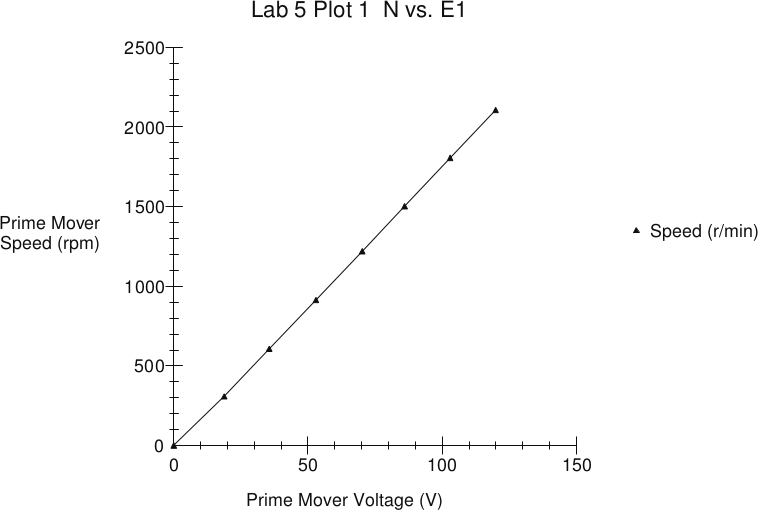
\includegraphics[width=\textwidth]{img/plot1}
  \caption{Prime Mover Speed vs. Prime Mover Voltage}
  \label{fig:plot_01}
\end{figure}

\begin{figure}[H]
  \centering
  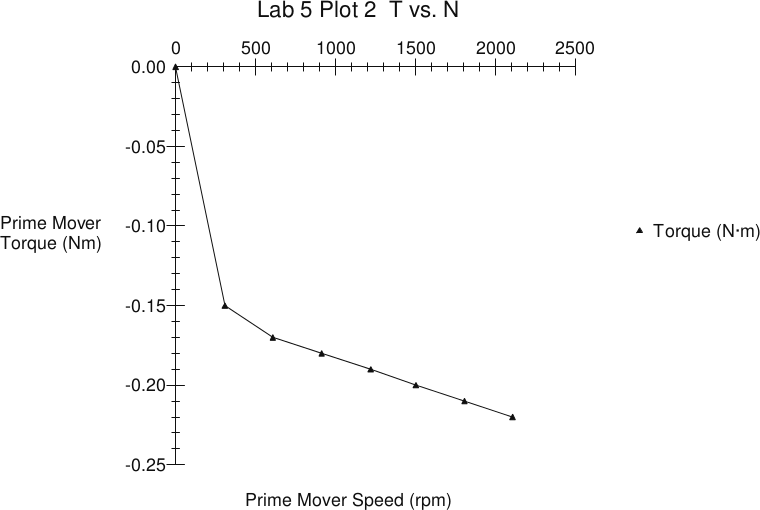
\includegraphics[width=\textwidth]{img/plot2}
  \caption{Prime Mover friction torque vs. Prime Mover Speed}
  \label{fig:plot_02}
\end{figure}

\subsection{Dynamometer Operation}

\begin{table}[H]
  \centering
  \begin{tabular}{*{5}{c}}
    $n$ rpm & $T_{DYN}$ N-m& $T_{PM}$ N-m & $T_{NC}$ N-m & $T_C$ N-m \\
    \hline
    1500 &   0 & -0.66 &  --- &  --- \\
    1500 & 2.0 & -2.26 & 1.76 & 2.33 \\
  \end{tabular}
  \caption{Prime Mover non-corrected and corrected torques}
  \label{tab:table_03}
\end{table}

\subsection{Motor Losses and Efficiency}

\begin{table}[H]
  \centering
  \begin{tabular}{*{2}{c}}
    $T_{C}$ N-m& $N$ rpm \\
    \hline
    1.31 & 1337  \\
  \end{tabular}
  \caption{Dynamometer speed and correceted output torque for a dyno torque of 1.0 Nm}
  \label{tab:table_04}
\end{table}

\begin{table}[H]
  \centering
  \begin{tabular}{*{4}{c}}
    & Measured & Calculated & Percent Deviation \\
    \hline
    $P_{mech}$ N-m & 182.2 & 183.4  & 0.65  \\
    $P_{in}$ N-m & 241.5 & --- & --- \\
    $P_{loss}$ N-m & 59.3 & --- & --- \\
    $\eta$ \% & 75.5 & 75.45 & 0.60 \\
  \end{tabular}
  \caption{Measured and calculated values for mechanical power output,
  electrical power input, and Prime Mover efficiency; computed Prime Mover
  power losses}
  \label{tab:table_05}
\end{table}

\begin{table}[H]
  \centering
  \begin{tabular}{*{7}{c}}
    \multicolumn{3}{c}{\textbf{Input}} & \multicolumn{3}{c}{\textbf{Output}}
    & \\

    \textbf{Voltage} & \textbf{Current} & \textbf{Electrical} &
    \textbf{Torque}  & \textbf{Speed}   & \textbf{Mechanical} &
    \textbf{Efficiency} \\

    &                  & \textbf{Power}      &
    &                  & \textbf{Power}
    & \\

    $E_1$ V          & $I_1$ I          & $PQS_1$ W           &
    $T$ N-m          & $N$ rpm          & $P_{m}$ W           &
    $A$ $\eta$ \\

    \hline

    88.71 & 0.94 &  89.90 & 0.32 & 1525.44 &  51.03 & 56.76 \\
    87.42 & 1.25 & 116.22 & 0.48 & 1474.08 &  74.44 & 64.05 \\
    86.08 & 1.58 & 144.32 & 0.67 & 1436.68 & 100.54 & 69.67 \\
    84.88 & 2.02 & 180.53 & 0.90 & 1394.14 & 131.70 & 72.96 \\
    83.98 & 2.40 & 210.73 & 1.11 & 1362.04 & 158.61 & 75.27 \\
    83.21 & 2.77 & 239.24 & 1.31 & 1340.72 & 183.39 & 76.65 \\
    82.42 & 3.13 & 267.18 & 1.50 & 1309.10 & 205.88 & 77.06 \\
    81.67 & 3.53 & 297.42 & 1.71 & 1273.63 & 227.89 & 76.62 \\
    81.01 & 3.90 & 325.22 & 1.92 & 1256.24 & 252.54 & 77.65 \\
    80.34 & 4.24 & 349.83 & 2.08 & 1232.10 & 268.29 & 76.69 \\
    79.57 & 4.64 & 379.02 & 2.30 & 1208.88 & 291.42 & 76.89 \\
  \end{tabular}
  \caption{Recorded values as the Dynamometer's torque was increased}
  \label{tab:table_06}
\end{table}

\begin{figure}[H]
  \centering
  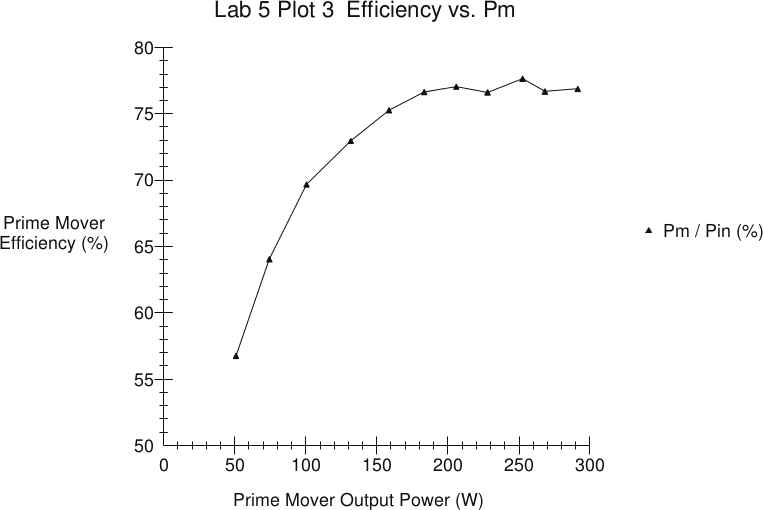
\includegraphics[width=\textwidth]{img/plot3}
  \caption{Prime Mover efficiency vs.\ mechanical output power}
  \label{fig:plot_03}
\end{figure}

\section{Conclusions} In Figure~\ref{fig:plot_02}, as the Prime Mover was first
starting to increase there was a large increase in torque in the opposite
direction of motion. However, as the Prime Mover gained rotational speed, the
opposition torque continued to increase but at a slower rate. In
Figure~\ref{fig:plot_03}, as the mechanical output power increased, the
efficiency also increased. This was because of the relationship between output
power and input power. As the output power became closer to the value of the
input power, then the efficiency of the motor became closer to 1.

In Part 2, when the Dynamometer was connected to the Prime Mover, the Prime
Mover generated a larger torque than it generated without the Dynanometer. This
was because of the added belt frition and friction torque of the Dyno bearings.
When the Dyno was set to genearate its own magnetic torque of 2 Nm, the Prime
Mover rotational speed decreased and thus its opposition torque in the opposite
direction of motion increased. The non-corrected torque generated by the Prime
Mover was without the loading of the Dyno taken into account. When the the
corrected torque was generated, the Dyno loading was taken into account and
thus this value represented the true torque produced by the Prime Mover. The
corrected torque was greater than the non-corrected torque by approximately the
same amount that the Prime Mover generated when the Dyno had not produced its
own magnetic torque.

In Part 3, the current was being increased because the PM/Dyno was set up as a
motor. As the torque produced by the Dyno increased, the voltage produced by
the Prime Mover decreased. However, the current increased as the Prime Mover
rotational speed decreased. The mechanical output power was less than the
electrical input power.  Electric power was being converted to mechanical
power.

\section*{Equations}

\[P_{mech}\ = \left( \frac{60}{2\pi} \right) (n \cdot T)\]
\[P_{loss} = P_{in} - P_{mech}\]

\section*{Circuits Tested}

\begin{figure}[H]
  \centering
  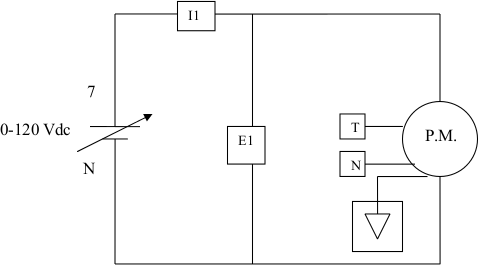
\includegraphics[width=0.8\textwidth]{img/circuit_01}
  \caption{Prime Mover Circuit}
  \label{fig:circuit_01}
\end{figure}

\begin{figure}[H]
  \centering
  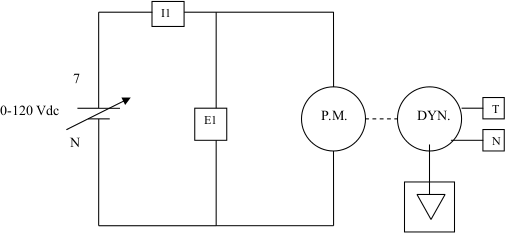
\includegraphics[width=0.8\textwidth]{img/circuit_02}
  \caption{Prime Mover Coupled to the Dynanometer}
  \label{fig:circuit_02}
\end{figure}

\end{document}
